\documentclass[12pt]{report}

\usepackage{color}
\usepackage[english]{babel}
\usepackage[utf8]{inputenc}
\usepackage{graphicx}
\usepackage{verbatim}
\usepackage{listings}
\usepackage{url}
\usepackage{stringenc}
\usepackage{pdfescape}
\usepackage{subfig}
\usepackage{float}
\usepackage{csquotes}  
\usepackage{tabularx}  
\usepackage[toc,page]{appendix}
\usepackage{caption}
\usepackage{titlesec}
\titleformat{\chapter}{\normalfont\huge}{\thechapter.}{20pt}{\huge\bf}
\usepackage[nottoc,notlof,notlot]{tocbibind} 
\setcounter{secnumdepth}{3}
\setcounter{tocdepth}{3} 

%%% Maketitle metadata
\newcommand{\horrule}[1]{\rule{\linewidth}{#1}} 	% Horizontal rule

\title{
\huge{\textbf{\textit{aWareHouse}}}\linebreak
\Large\textbf{\\Environment Control System for Warehouses}\linebreak\linebreak\linebreak

\includegraphics[width=8cm]{feup.pdf}\linebreak \linebreak
\large{MSc in Informatics and Computer Engineering} \linebreak
\large{Programming Paradigms \\ EIC0065-2S}\linebreak
}

\author{
Duarte Nuno Pereira Duarte - 201109179 (ei11101@fe.up.pt)\\
Hugo José Freixo Rodrigues - 201108059 (ei11086@fe.up.pt)\\
João Pedro Matos Teixeira Dias - 201106781 (ei11137@fe.up.pt)\\
\\
\\ Faculdade de Engenharia da Universidade do Porto \\ Rua Roberto Frias, s\/n, 4200-465 Porto, Portugal
}
 
\date{\today}
\begin{document}
\clearpage\maketitle
\thispagestyle{empty}
%************************************************************************************************
%************************************************************************************************

\newpage
\section*{Abstract}

We are in the rise of IoT (Internet of Things). A world where everything is connected and we can, with simple tools, monitor and control everything. In this context, there is a lot of room to a more recurrent use of different programming paradigms: from the hardware to the cloud, there is a need to interact with many different layers of system architecture for a single application.

Our application, \textit{aWareHouse}, was designed with the objective of, with a simple interface, we can monitor a house or a warehouse in terms of environment conditions (temperature, humidity, sound and luminosity). 

To accomplish this we used a combination of hardware/software and different programming languages, in a way that gave us a robust application that can be used to configure a warning system when there are changes in the environment, to take decisions analysing the past conditions and the relations with external (meteorological) conditions or simply to monitor the current conditions inside our warehouse.


\newpage
%************************************************************************************************
%************************************************************************************************
\tableofcontents
%************************************************************************************************
%************************************************************************************************
\newpage

\chapter{Introduction}

The \textit{aWareHouse} project was developed for the Programming Paradigms course unit of the Master in Informatics and Computing Engineering at FEUP. The project was developed with the objective of combining, at least, three programming paradigms in the same application.

The base motivation for this project was the Internet of Things, as defined by \textit{Gartner}:

\blockquote{The Internet of Things (IoT) is the network of physical objects that contain embedded technology to communicate and sense or interact with their internal states or the external environment.}

To achieve this we designed a low cost system capable of giving the user the possibility of, using a relative small hardware box, monitor the environment of a given place like a house or warehouse. This, associated with a system capable of maintain records of the past conditions of the environment (plus external weather conditions), results in one application that gives the user the capacity of making decisions, be aware of the environment status using alerts and see the current conditions.

As explained before, the capabilities of this application is a system useful in a lot of situations, e.g. the monitoring of a warehouse and verifying the relation between weather and internal conditions to make decision on what is the best settings for a refrigeration system and assure that the, for example, temperature is always below the maximum recommended. Another example is simple use it as a house control system and, for example, verify if someone forgot to turn any light off.

\newpage
\chapter{System Description}
\section{Conceptual Description}
\subsection{Functionalities}

\begin{figure}
    \centering
    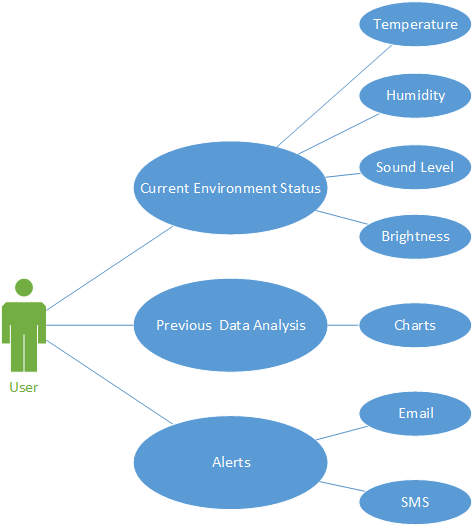
\includegraphics[scale=0.5]{use.png}
    \caption{Use Case diagram.}
    \label{fig:use}
\end{figure}

The \textit{aWarehouse} application consists in a system that scans the environment of the room where the sensors are placed and stores all the information about it on a time series database.

The system can read temperature, humidity, sound and luminosity values as described in \ref{fig:use}. Additionally user can define maximum and minimum values so the system will alert whenever an environment factor exceeds this range.
This way the user can have absolute control of the room where \textit{aWarehouse} is installed. This application can be very useful in a server room, with the temperature sensor the user can control the room temperature and prevent an overheating. With the sound sensor the user knows if someone is in the room and with the luminosity sensor the user can check if someone forgot to turn off the lights.



\subsection{Architecture}

\subsubsection{Physical Architecture}

\begin{figure}[H]
    \centering
    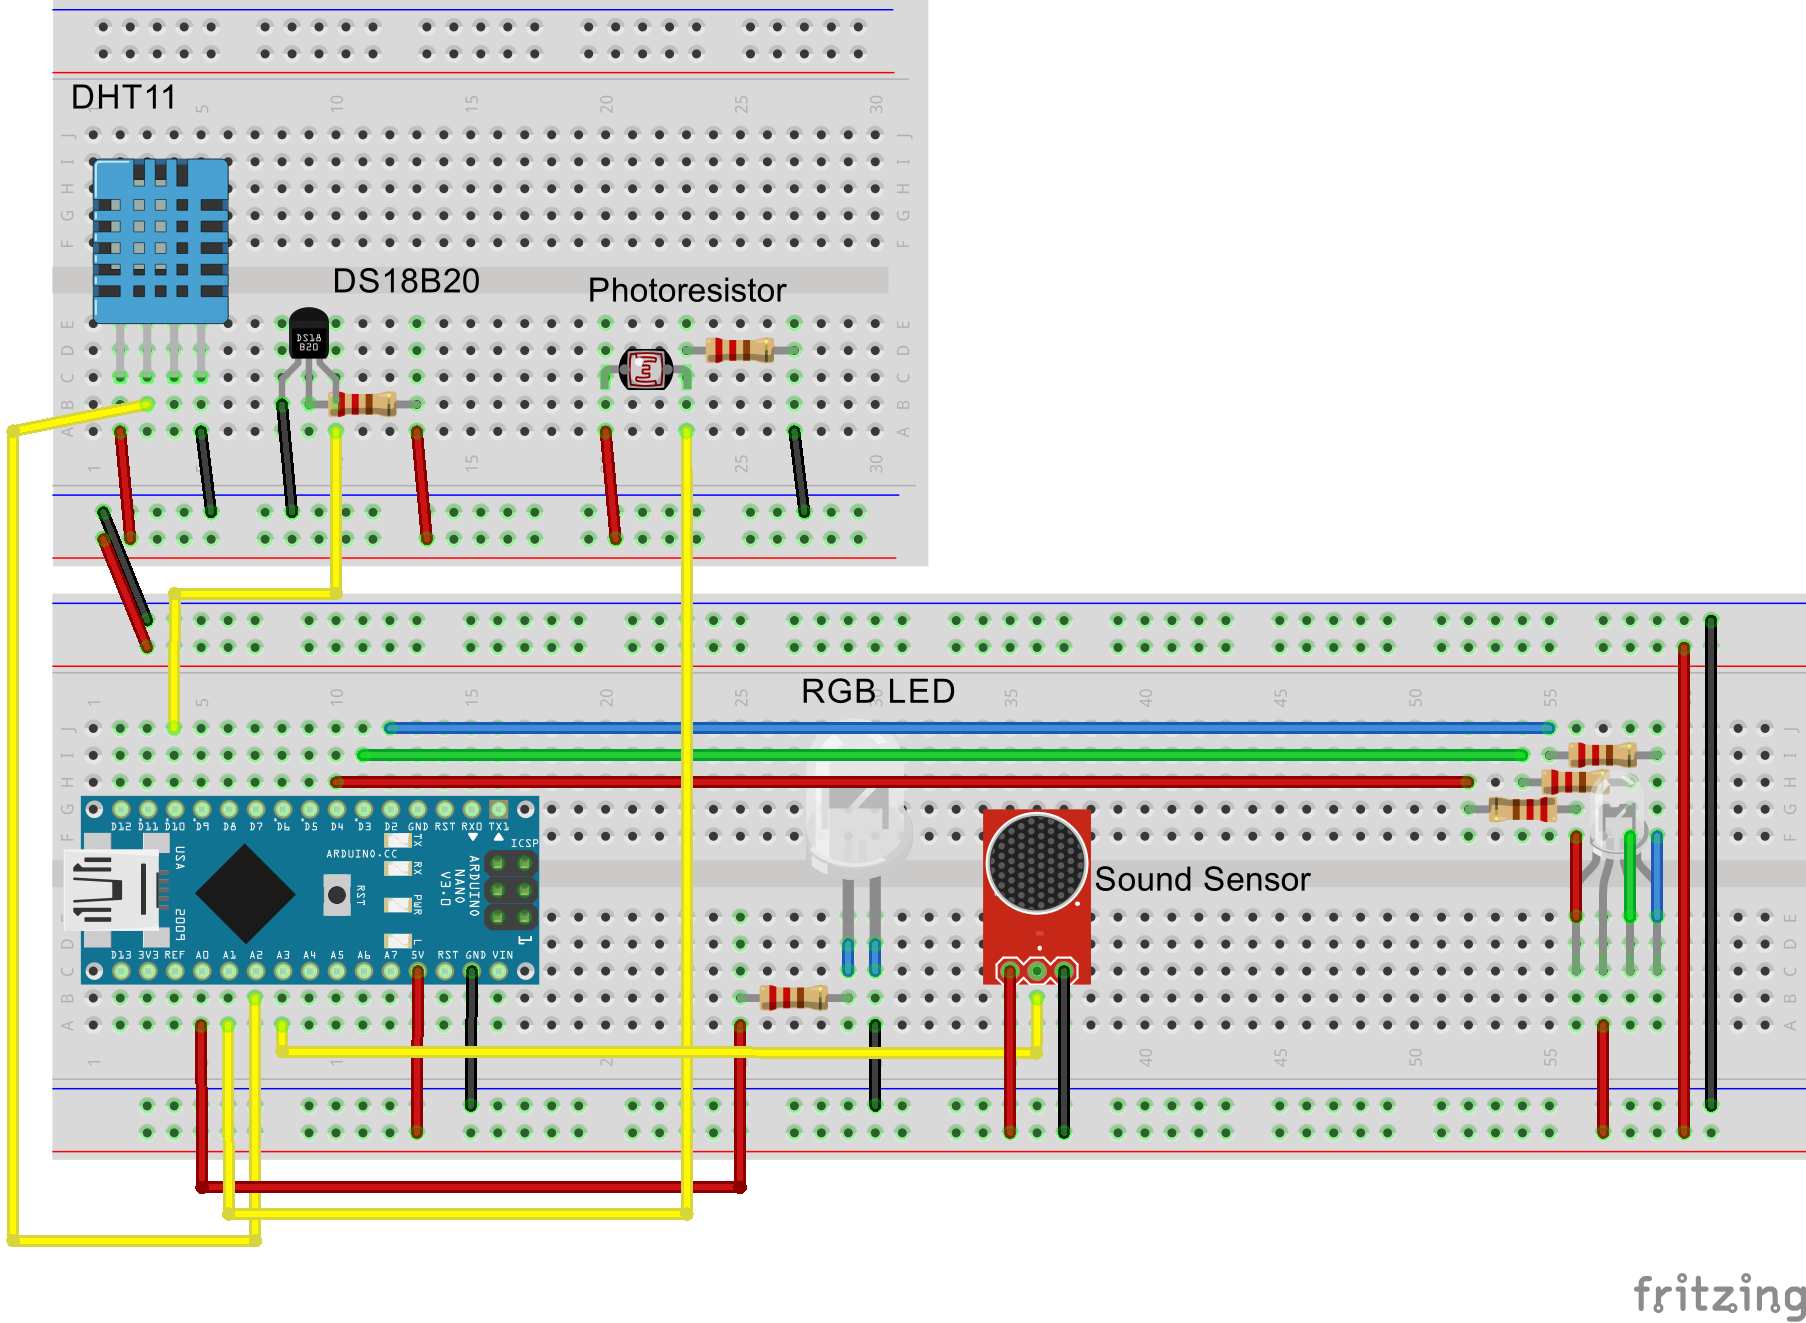
\includegraphics[width=0.8\textwidth]{schematics.png}
    \caption{Circuit diagram.}
    \label{fig:circ}
\end{figure}

\begin{table}[H]
\begin{tabularx}{\textwidth}{ |l|X|p{3cm}| }
  	\hline
  	\textbf{Sensor}  & \textbf{Description} & \textbf{Input/Output} \\
 	\hline
 	DHT11  & Basic and low-cost digital temperature and humidity sensor. It uses a capacitive humidity sensor and a thermistor to measure the surrounding air, and spits out a digital signal on the data pin. & Temperature and Humidity values. \\
 	\hline
 	DS18B20  & 1-wire digital temperature sensor fairly precise (+- 0.5ºC over much of the range) and can give up to 12 bits of precision from the onboard digital-to-analog converter. & Temperature values. \\
 	\hline
 	LM393 & One single channel output sound level. Low level output signal and when there is sound output low, lights lit. & Sound level values. \\
 	\hline
 	Diffused LED & A diffuse LED with with separate red, green and blue LED chips inside, capable of emitting a color-mix resulted of the values passed to each chip. & RGB Color or Color-Mix.\\
 	\hline
 	Photo cell & Photo cell or CdS photoresistor is a little light sensor. As the squiggly face is exposed to more light, the resistance goes down and the voltage goes up. & Voltage value.\\
 	\hline
\end{tabularx}
	\caption{Sensors description.}
  	\label{tab:prolangs}
\end{table}

\textbf{\\Arduino}

\begin{figure}[H]
    \centering
    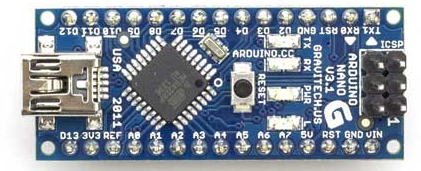
\includegraphics[width=0.5\textwidth]{img/arduino.png}
    \caption{Arduino micro-controller.}
    \label{fig:arduino}
\end{figure}

The Arduino Nano (fig.\ref{fig:arduino}) is a small, complete, and breadboard-friendly micro-controller based on the ATmega328 processor chip and works with a Mini-B USB cable for energy and data transfer. It has 32 KB of flash memory space of which 2 KB used by bootloader.

Each of the 14 digital pins on the Nano can be used as an input or output and 8 analog inputs, each of which provide 10 bits of resolution (i.e. 1024 different values). 

The Arduino provides an UART TTL (5V) serial communication, which is available on digital pins 0 (RX) and 1 (TX). An FTDI FT232RL on the board channels this serial communication over USB and the FTDI drivers (included with the Arduino software) provide a virtual COM port to software on the computer. 


\textbf{\\Raspberry Pi}

\begin{figure}[H]
    \centering
    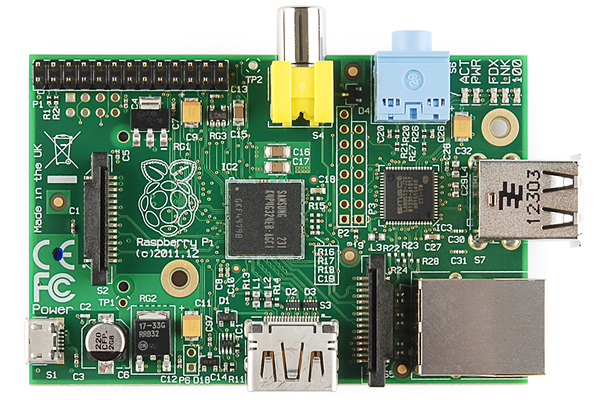
\includegraphics[width=0.5\textwidth]{img/rpi.png}
    \caption{Raspberry Pi 1 Model B.}
    \label{fig:rpi}
\end{figure}

The \textit{Raspberry Pi 1 Model B} (fig. \ref{fig:rpi}) is a single-board computer which can be used for many of the things that a desktop is used to.

The design is based around a Broadcom BCM2835 SoC, which includes an ARM1176JZF-S 700 MHz processor, VideoCore IV GPU, and 512 Megabytes of RAM. The memory used is a SD card for booting and long-term storage. This board is intended to run Linux kernel based operating systems. Additionally this has two USB ports and a 10/100 Ethernet controller.

\subsubsection{Logic Architecture}

\begin{figure}[H]
    \centering
    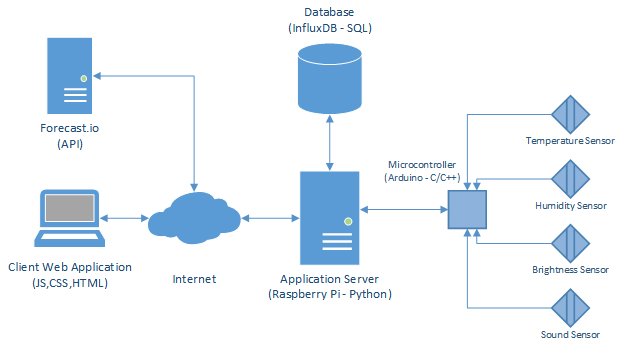
\includegraphics[width=0.9\textwidth]{arc.png}
    \caption{Architecture diagram.}
    \label{fig:arc}
\end{figure}

The application base logic architecture, as presented in fig. \ref{fig:arc}, is divided in three principal layers, the low-level layer were the sensors are controlled, the back-end layer were all the data and services are managed, and the front-end layer which is dashboard web application.

Although the Raspberry Pi has a GPIO port (General Purpose Input/Output) capable of interact with the sensors we used, we opted for using a separated controller, an Arduino, for doing that. This is motivated by the need of a real-time system on reading the sensors and there's too much running in Linux to get that kind of accuracy. The Linux kernel dispatcher isn't made to support real-time since there's a massive number of tasks that you simply can't run without.

\subsection{Programming Languages and Technologies}

In the context of realizing this project we conciliated a diversity of technologies and programming languages that, working together in the architecture presented at fig. \ref{fig:arc}, made the application possible. Starting by enumerating the programming languages used and the reasons for choosing those languages are the following.
\begin{itemize}
\item Arduino Language\cite{arduinolang} is a low level language based on C/C++ and integrated with AVR Libc\cite{avr} and allows the use of any of its functions for interacting with hardware. Since its a derivative language of C/C++ it has a multi-paradigm design being imperative and object-oriented. The version used is v1.6.4. 
\begin{itemize}
\item DHT Sensor Library\cite{dhtada} is an Arduino library for the DHT series of low cost temperature/humidity sensors that facilitates the reading of values from these sensors.
\item OneWire Library\cite{pjrc} is used to access 1-wire devices made by Maxim/Dallas, such as temperature sensors. For temperature sensors, witch is our case, the DallasTemperature\cite{dallas} library can be used with this library.
\end{itemize}
\item Python Language\cite{pylang} is a general-purpose, high-level programming language. Python supports multiple programming paradigms, including object-oriented, imperative and functional programming. It features a dynamic type system and automatic memory management and has a large and comprehensive standard library. The version used is v2.7.9.
\begin{itemize}
\item Flask Library\cite{flask} is a micro web application framework for creating simple web RESTful applications.
\item Schedule Library\cite{schedule} makes possible to run Python functions (or any other callable) periodically at pre-determined intervals using a simple, human-friendly syntax.
\item pySerial Libray\cite{pyserial} facilitates the use of serial port communication in Python applications.
\end{itemize}
\item Web Languages\cite{moz} are a set of languages that are interpreted by a browser in a rendering process to present the content on a browser screen. 
\begin{itemize}
\item HTML5 or HyperText Markup Language is the language used to describe and define the content of a Web page in a structured format.
\item JavaScript(ECMAScript 5/6) is the programming language that runs in the browser, which is used to build advanced user interactive Web sites and applications.
\item CSS3 or Cascading Style Sheets are used to describe the appearance of Web content.
\end{itemize}
\item SQL or Structured Query Language is a special-purpose programming language designed for managing data held in databases. In our case, InfluxDB database, has a SQL like query language\cite{influxkey} for find and grouping data.

\end{itemize}

In addiction to the programming languages we used a set of technologies as a part of our application as presented in table \ref{tab:tech}.

\begin{table}[H]
\begin{tabularx}{\textwidth}{ |l|X| }
  	\hline
  	InfluxDB & InfluxDB\cite{influx} is a time series, metrics, and analytics database. It’s written in Go and its oriented for recording events data, like data from sensors.\\
 	\hline
 	Grafana & Grafana\cite{grafana} is an open-source metrics dashboard with direct integration with various databases like InfluxDB.\\
  	\hline
 	Web API's &\begin{itemize}
 	\item Forecast.io: Weather forecast RESTful API that returns the current weather conditions for a specific location (Latitude, Longitude)
 	\item Twilio: Simple RESTful API for sending text messages (SMS).
 	\item Mandrill: Powerful, scalable, and affordable email infrastructure as a service, using a RESTful API: 
 	\end{itemize}   \\
	\hline
\end{tabularx}
	\caption{Technologies.}
  	\label{tab:tech}
\end{table}

\section{Implementation Description}

\subsection{Implementation Details}

This project had the need of using and establishing a diversity of APIs (Application Programming Interface) for communicating between the different application layers and external services.

On one hand, we used various RESTful API for accessing external services (Mandrill\cite{mandrillapi}, Forecast.io\cite{fcapi} and Twilio\cite{twilioapi}) as refereed in table \ref{tab:tech}. The RESTful stands for Representational State Transfer, that consists in using the standard HTTP operations for communication data in JSON or XML format. In our case, the external services used can communicate using JSON (JavaScript Object Notation) messages for requesting and pushing data.

Additionally we standardize a REST API for communicating with the Python server from our web application.

On the other hand, for establishing communication between the Python server and the Arduino we used the Serial Port communication using the Arduino serial port\cite{serial}, and a Python library called \textit{pySerial}\cite{pyserial}. For this we standardized a system of request/response were we passed a character that expressed the operation wanted and the Arduino responded using a JSON string with the values requested. The serial port communication is emulated above an USB port.



\subsection{Development Environment}

The development environment used depended on the layer that we were working, because different languages/technologies required different environments.

For developing the low level hardware phase, using the Arduino platform, we needed to use the Arduino Software (IDE)\cite{arduinoide}, that compiles the Arduino code, checks for errors and uploads it to the Arduino Board.

When developing the Python server application we used the Python compiler for analysing Python source code and generating Python bytecode, and the Python IDLE that is the Python IDE built with the Tkinter GUI toolkit. Beside this, when deploying the Python server code on the Raspberry Pi we used  SSH (Secure Shell) to connect with it and initiating text-based shell session on the remote machines in a secure way, allowing us to run commands on the machine prompt without the need of being physically present near to the machine.

Another tool that we needed was the Go language compiler (v1.4) since we used InfluxDB which is written in Go Lang\cite{goinflux}, and we needed to compile it for ARM processor (Raspberry Pi processor architecture).

For developing the client web application and extending the Grafana we used a text editor.

Additionally we used Git control version system for sharing/working with code between the members of the working team associated with the GitHub free repository system for students.
\newpage
\chapter{User Interface}
\begin{figure}[H]
    \centering
    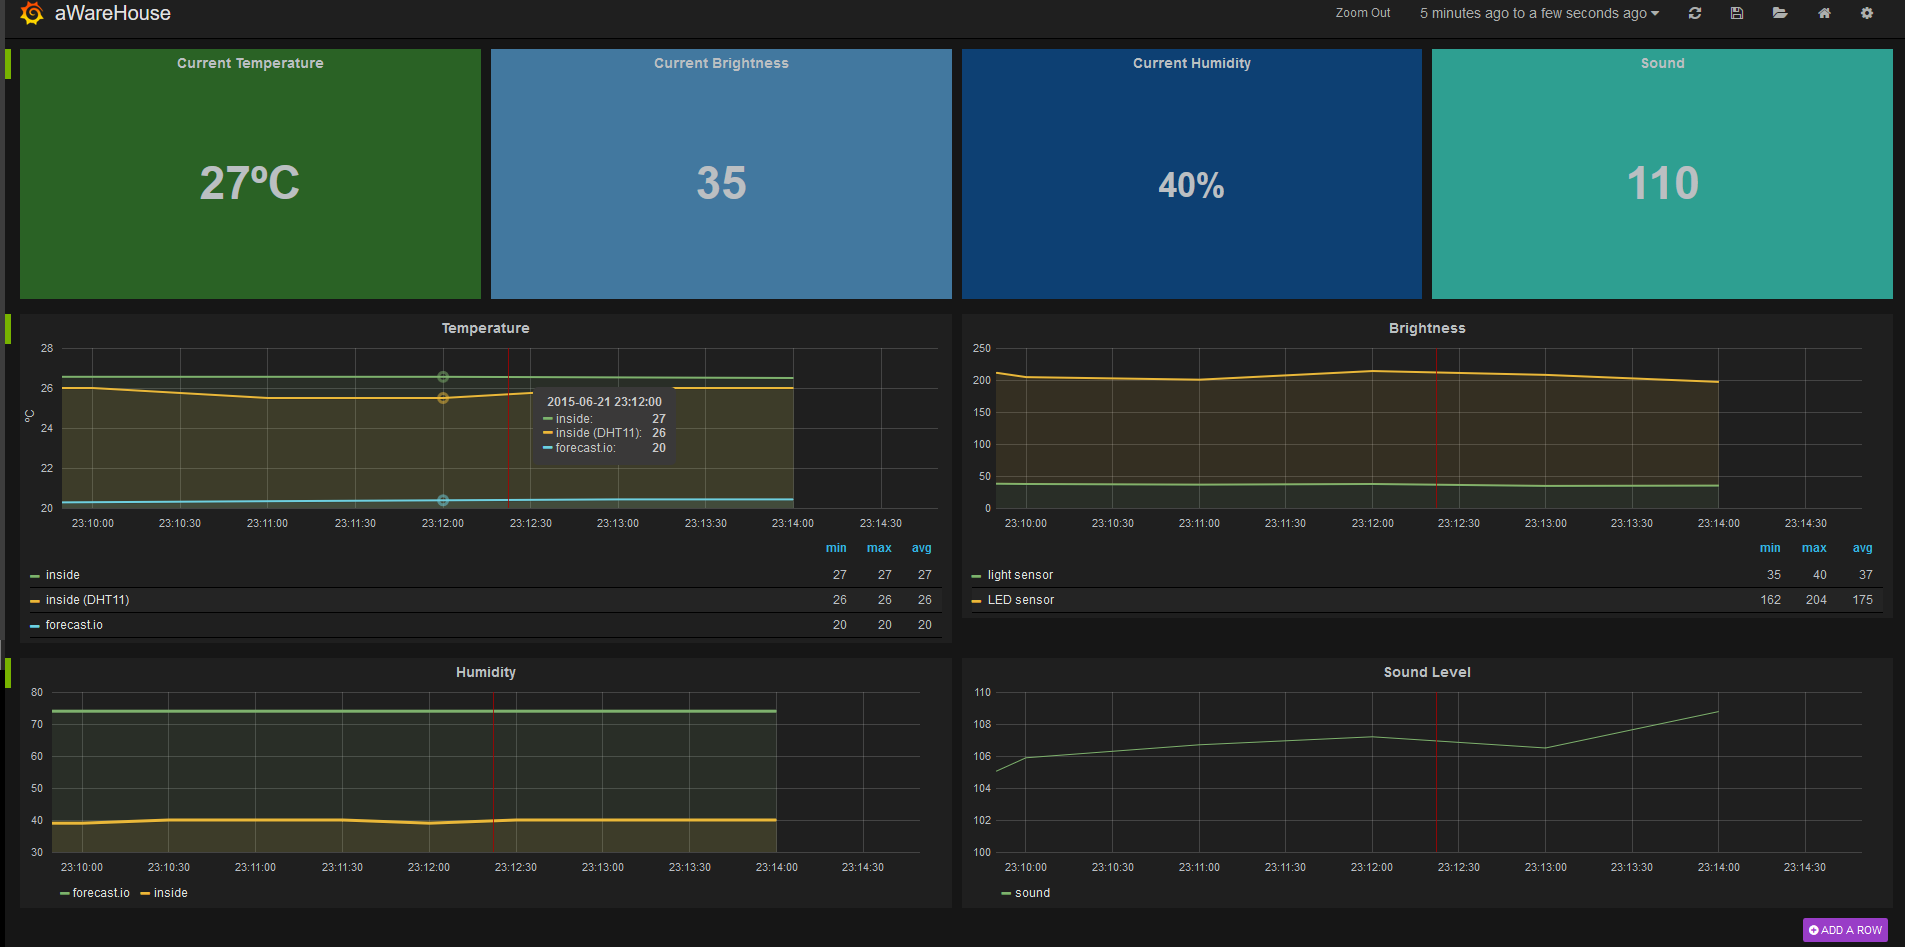
\includegraphics[width=0.8\textwidth]{img/main.png}
    \caption{aWareHouse dashboard.}
    \label{fig:main}
\end{figure}
\begin{figure}[H]
    \centering
    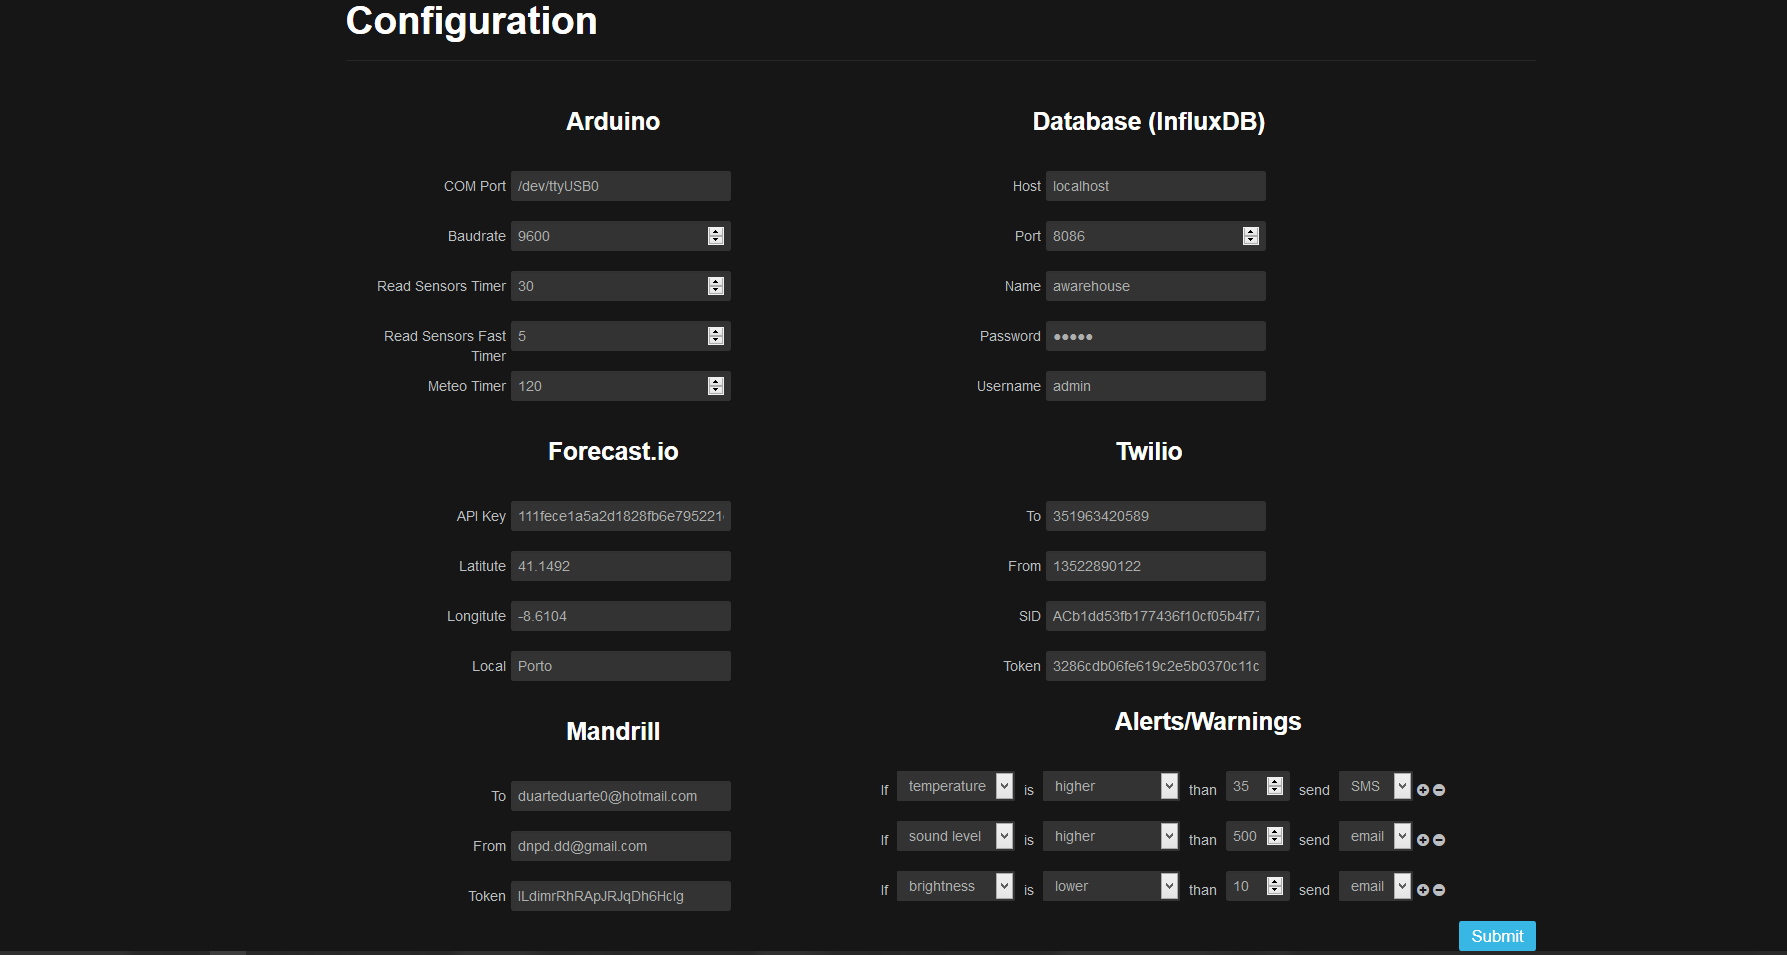
\includegraphics[width=0.8\textwidth]{img/config.png}
    \caption{Configuration window.}
    \label{fig:config}
\end{figure}

\newpage
\chapter{Conclusion}

The \textit{aWareHouse} project was designed to take advantage of different programming paradigms in a way that resulted in a stable product, using various programming languages, frameworks, libraries and technologies. 

In a way of summary, we used low-level programming for Arduino and sensors, taking advantages of imperative paradigm. For the server that communicates with the web application and the Arduino we used Python that is a multi-paradigm language (object-oriented, imperative and functional). For the web application itself we used the standard web technologies (JavaScript, HTML and CSS). JavaScript, principally, is know for being another multi-paradigm language (scripting, object-oriented with prototypes, imperative and functional).

The actual result was a solution that can easily adapted for the market with a relative good precision, trustability and stability. Additionally it is easy adaptable and/or extendible with new functionalities (e.g more sensors).

This project fits in a time that we start to hear everyday more about \textit{Internet of Things} and \textit{Big Data}, and the possibilities that this brings to us. We conciliated this two big thematics and give the user the power to watch and be aware of a warehouse or any confined space, and, at the same time, be capable of see the past data and the influence of external conditions in inside environment.

\newpage
\chapter{Improvements}

Although we think that \textit{aWareHouse} is almost ready to market at this stage, we already found space for improvement and evolution, namely:
\begin{itemize}
 \item Addition of more and basic sensors like, for example, a motion sensor.
 \item The storage system has to be improved because it slows down with the  accumulation of past data.
 \item Possibility to integrate some automatic advice system, using artificial intelligence, that provides the user advices on what to change to achieve certain goals (e.g colder rooms, reduce eletrical costs, etc.).
 \item Improve the security of application by restricting access and better data protection.
\end{itemize} 

We see this points as growing space, and possibility to make a better application for the final user.

\renewcommand\bibname{References}
\begin{thebibliography}{}

\bibitem{twilioapi}
  \emph{Twilio REST Web Service Interface},
  \url{http://www.twilio.com/docs/api/rest}
  
\bibitem{fcapi}
  \emph{The Dark Sky Forecast API},
  \url{http://developer.forecast.io/docs/v2}
  
\bibitem{mandrillapi}
  \emph{Mandrill API Documentation},
  \url{http://mandrillapp.com/api/docs}
  
\bibitem{serial}
  Arduino, \emph{Serial},
  \url{http://www.arduino.cc/en/reference/serial}
  
\bibitem{pyserial}
  \textit{pySerial}, \emph{pySerial’s documentation},
  \url{http://pyserial.sourceforge.net/}
  
\bibitem{influx}
  \textit{InfluxDB}, \emph{An open-source, distributed, time series database
with no external dependencies},
  \url{http://influxdb.com/}
  
\bibitem{grafana}
  \textit{Grafana}, \emph{An open source, feature rich metrics dashboard and graph editor for
Graphite, InfluxDB \& OpenTSDB},
  \url{http://grafana.org/}
  
\bibitem{dallas}
  \textit{Dallas Temperature Control Library},
  \url{http://milesburton.com/Main_Page?title=Dallas_Temperature_Control_Library}
  
\bibitem{dhtada}
  \textit{Using a DHTxx Sensor}, Adafruit Industries,
  \url{https://learn.adafruit.com/dht/using-a-dhtxx-sensor}
  
\bibitem{pjrc}
  \textit{OneWire Library}, Jim Studt,
  \url{http://www.pjrc.com/teensy/td_libs_OneWire.html}, 2007
  
\bibitem{flask}
  \textit{Flaks}, Armin Ronacher,
  \url{http://flask.pocoo.org/}, 2014

\bibitem{schedule}
  \textit{Python job scheduling for humans}, Daniel Bader,
  \url{https://github.com/dbader/schedule}
  
\bibitem{arduinolang}
  \textit{Arduino Language Reference},
  \url{http://www.arduino.cc/en/Reference/HomePage}
  
\bibitem{avr}
  \textit{AVR Libc Modules},
  \url{http://www.nongnu.org/avr-libc/user-manual/modules.html}
  
\bibitem{pylang}
  \textit{Python},
  \url{https://www.python.org/}
  
\bibitem{influxkey}
  \textit{InfluxDB Query Language},
  \url{http://influxdb.com/docs/v0.8/api/query_language.html}
  
\bibitem{moz}
  \textit{Web technology for developers}, Mozilla Developer Network,
  \url{https://developer.mozilla.org/en-US/docs/Web}
  
\bibitem{arduinoide}
  \textit{Arduino Software}, Arduino,
  \url{http://www.arduino.cc/en/Main/Software}, 2015
 
\bibitem{goinflux}
  \textit{Contributing InfluxDB}, InfluxDB,
  \url{https://github.com/influxdb/influxdb/blob/master/CONTRIBUTING.md}, 2015
\end{thebibliography}

\newpage

\begin{appendices}
\chapter{Appendix}
\section{Hardware}
\subsection*{Raspberry Pi}

Technical Specs:
\begin{itemize}
\item Chip: Broadcom BCM2835 SoC full HD multimedia applications processor
\item CPU: 700 MHz Low Power ARM1176JZ-F Applications Processor
\item GPU: Dual Core VideoCore IV® Multimedia Co-Processor
\item Memory: 512MB SDRAM
\item Ethernet: onboard 10/100 Ethernet RJ45 jack
\item USB: 2.0 Dual USB Connector
\item Video Output: HDMI (rev 1.3 \& 1.4) Composite RCA (PAL and NTSC)
\item Audio Output: 3.5mm jack, HDMI
\item Onboard Storage: SD, MMC, SDIO card slot
\item Operating System: Linux (Raspbian OS)
\item Dimensions: 8.6cm x 5.4cm x 1.7cm
\end{itemize}

\subsection*{Arduino}

Technical Specs:
\begin{itemize}
\item Microcontroller: Atmel ATmega328
\item Operating Voltage (logic level): 5 V
\item Input Voltage (recommended): 7-12 V
\item Input Voltage (limits): 6-20 V
\item Digital I/O Pins: 14 (of which 6 provide PWM output)
\item Analog Input Pins: 8
\item DC Current per I/O Pin: 40 mA
\item Flash Memory:	32 KB of which 2 KB used by bootloader
\item SRAM: 2 KB 
\item EEPROM: 1 KB
\item Clock Speed: 16 MHz
\item Dimensions: 0.73" x 1.70"
\item Length: 45 mm
\item Width: 18 mm
\item Weigth: 5 g
\end{itemize}
\subsection*{Sensor DHT11}
Technical specs:
\begin{itemize}
\item 3 to 5V power and I/O
\item 2.5mA max current use during conversion (while requesting data)
\item Good for 20-80\% humidity readings with 5\% accuracy
\item Good for 0-50ºC temperature readings +- 2ºC accuracy
\item No more than 1 Hz sampling rate (once every second)
\item Body size 15.5mm x 12mm x 5.5mm
\item 4 pins with 0.1" spacing
\end{itemize}

\subsection*{Sensor DS18B20}
Technical specs:
\begin{itemize}
\item Usable temperature range: -55 to 125 ºC (-67F to +257F)
\item 9 to 12 bit selectable resolution
\item Uses 1-Wire interface- requires only one digital pin for communication
\item Unique 64 bit ID burned into chip
\item Multiple sensors can share one pin
\item +-0.5C Accuracy from -10ºC to +85ºC
\item Temperature-limit alarm system
\item Query time is less than 750ms
\item Usable with 3.0V to 5.5V power/data
\end{itemize}
\subsection*{Sound Sensor (LM393)}
Technical specs:
\begin{itemize}
\item LM393 Controller
\item Electret microphone
\item Working voltage: DC 4 - 6 V
\item With a signal output instruction
\item One single channel output
\item Low level output signal
\item When there is sound output low, lights lit
\end{itemize}
\subsection*{Diffused Led}
Technical specs:
\begin{itemize}
\item 10mm diameter
\item Red: 623 nm wavelength, Green: 523 nm, Blue: 467 nm
\item Red: 1.8-2.2V Forward Voltage, at 20mA current, Green: 3.0-3.4V, Blue: 3.0-3.4V
\item 50 degree viewing angle.
\item Red: 700 mcd typical brightness, Green: 2100 mcd, Blue: 900 mcd
\end{itemize}
\subsection*{Photo cell (CdS photoresistor)}
Technical specs:
\begin{itemize}
\item When its light, the resistance is about 5-10KOhm, when dark it goes up to 200KOhm.
\item The voltage on the pin will be 2.5V or higher when its light out and near ground when its dark.
\end{itemize}
\end{appendices}

\end{document}
